\clearpage
\chapter{Genetic Algorithms}\label{chap:geneticAlgorithms}

Genetic algorithms are used to model optimization problems and to find solutions
to those problems using techniques borrowed from natural
evolution~\cite{Holland1992,goldberg1989genetic,fogel2000evolutionary}. In
nature, populations of individuals exist in some environment. Individuals that
are more fit in their environment are more likely to survive to pass on their
genes to new individuals, leading to the overall population being more fit.

Likewise in genetic algorithms there are populations of solutions. Those
solutions that are more fit in the solution space are more likely to pass their
genes to a new population either through reproduction, recombination, or
mutation. Over time, the population tends to have more fit solutions.

Genetic algorithms can be used to find approximate solutions to problems that
are considered to be intractable.

We begin with a very brief summary of the complexity class
NP~\cite{alsuwaiyel1999algorithms,Cormen:2009:IAT:1614191} and list some
examples of those types of problems. There are various ways to tackle NP
problems such as approximation, the Monte Carlo method, and
heuristics~\cite{russell2010artificial}. None of those methods can guarantee an
exact solution, just a ``good enough'' solution.

Another way to get an approximate solution is to use a genetic algorithm. A
genetic algorithm is similar to the Monte Carlo method, in that a set of
solutions is created randomly. But unlike randomization, we do not continue to
generate more random solutions in the hopes of stumbling on a better solution.
The development of better solutions in a genetic algorithm is guided by
selection pressures which eliminate poor solutions and evolve good solutions
into better solutions.

After looking at the basic genetic algorithm, we briefly discuss various ways to
modify the standard genetic algorithm to expand its ability to find solutions to
problems. These enhancements allow genetic algorithms to be applied to a large
set of problems.

\section{NP Problems}

In complexity theory, there are a number of classes that are used to categorize
problems~\cite{alsuwaiyel1999algorithms,Cormen:2009:IAT:1614191}. The simplest
of those classes is the class P: those problems which can be deterministically
solved in polynomial time. Using big O notation, we write

\(P \in O(n^{k})\)

where \(n\) is the size of the problem, \(k\) is some constant, and the
notation \(O()\) refers to the time complexity of the problem.

A very brief subset of problems that are in the P complexity class are listed
below~\cite{greenlaw1991compendium}.

\begin{itemize}
\item{Linear programming - Maximize a linear function subject to linear
inequality constraints.} 
\item{Context Free Grammar Membership - Given a context-free grammar and a
string, can that string be generated by that grammar?}
\item {2-Player Game - Given a 2-player game, is the starting position \(s\) a
winnning position for player \(P_1\)?}
%\item {Prime membership - Given some number \(n\), is \(n\) a prime number?}
\end{itemize}

However, there are some problems which (so far) do not have a solution that can
be deterministically computed in polynomial time. In \emph{Algorithms: Design
Techniques and Analysis}~\cite{alsuwaiyel1999algorithms}, NP problems are
defined as ``\ldots those decision problems for which there exists a
nondeterministic algorithm that runs in polynomial time.'' Cormen et al, provide
this simple definition of NP: ``The class NP consists of those problems that are
`verifiable' in polynomial time~\cite{Cormen:2009:IAT:1614191}.'' By combining
those definitions we can say there are some problems for which no deterministic
algorithm has yet been found which can produce an exact or optimal solution in
polynomial time. However, there may be nondeterministic algorithms which can
produce a solution in polynomial time. If a solution to such a problem is
produced by a nondeterministic algorithm, and the solution can be verified by a
deterministic algorithm in polynomial time, then the problem is a member of the
class NP\footnote{NP problems can be further classified into additional
classes such as NP-Hard and NP-Complete. However, for the purposes of this
chapter the two classes P and NP are sufficient. Interested readers can find
more information in any reference on algorithms, including the references cited
above, \emph{Algorithms: Design Techniques and Analysis} by M. H.
Alsuwaiyel~\cite{alsuwaiyel1999algorithms} and \emph{Introduction to Algorithms}
by Cormen et al~\cite{Cormen:2009:IAT:1614191}.}.

A very brief list of some problems that are in the NP complexity class are
below~\cite{garey1979computers}.

\begin{itemize}
\item{Integer factorization decision problem - given integers \(n\) and \(k\),
is there a factor \(f\) with \(1 < f < k\) and \(f\) dividing \(n\)?}
\item{Graph isomorphism - given two different graphs, can they be drawn
identically?}
\item{Traveling salesman decision problem - is there a route of given length
\(k\) that goes through all the nodes in a certain network?}
\end{itemize}

In attempting to solve some of these NP problems, researchers have developed a
number of nondeterministic techniques that can be used to find ``good enough''
answers. That is, techniques that can find some solution relatively quickly,
where the solution approaches the optimal solution within a few percentage
points. This ``good enough'' solution may even be the optimal solution, although
there is no guarantee that it is optimal. Some of these techniques are
approximation, the Monte Carlo method, and
heuristics~\cite{Cormen:2009:IAT:1614191,russell2010artificial}.

\begin{itemize}
  \item {Approximation - Use an algorithm that runs in polynomial time that is
  able to find solutions that are within a factor of \(\rho (n)\) of the cost of
  the optimal solution.}
  \item {Monte Carlo - Solutions are generated randomly. After some amount of
  time, the best solution so far is chosen as the result.}
  \item {Heuristics - Use a rule of thumb that guides the algorithm to a
  solution that is close to the optimal solution.}
\end{itemize}

Approximation and heuristics can find solutions, but because they may not
explore the entire the search space it is possible that they may never produce
highly optimal solutions. The Monte Carlo method can explore large regions of
the search space, but because of its random nature it may require the
generation of a large amount of solutions before it finds one that is close to
optimal.

Genetic algorithms combine the random nature of the Monte Carlo method to
explore large regions of the search space with guidance that is analogous to
heuristics to find near optimal solutions with relatively low time cost.

\section{Basic Genetic Algorithms}

Genetic algorithms~\cite{Holland1992, goldberg1989genetic,
fogel2000evolutionary, haupt2004practical} tend to be good at solving
optimization problems where the solution has the following two attributes:

\begin{enumerate}
  \item {The solution can be encoded into some kind of data structure.}
  \item {There is a relatively low cost deterministic method to measure the
  fitness (the ``goodness'') of the solution.}
\end{enumerate}

A genetic algorithm consists of randomly creating solutions to a problem, and
encoding those solutions into a data structure. The quality of those solutions
is assessed, and then new solutions are created by reproducing, combining, or
mutating the current set of solutions into a new set. Higher quality solutions
are reproduced, combined, or mutated with higher probability than lower quality
solutions. Since higher quality solutions are more likely to propagate into the
next generation, over time they come to make up larger proportions of the
population. Combination and mutation introduce variations into the population
which creates solutions which cover unexplored regions of the solution space and
make it more likely that solutions don't get trapped in local minima or maxima.
Over time this tends to produce approximate solutions which are optimal or very
close to optimal.

To use the techniques of a genetic algorithm the solution to the problem needs
to be represented in a data structure that can be manipulated using evolutionary
techniques. This means that it is relatively easy to initialize a population of
data structures that represent possible solutions, relatively easy to measure
the fitness of the solution, and relatively easy to modify the starting
population into a new population. These features map onto the general flow of a
genetic algorithm which is illustrated in Figure~\ref{figure-gaflow}. A brief,
high-level overview of genetic algorithms is given in the sections that follow.
The summary in the remainder of this section is based on the work of
Holland~\cite{Holland1992}, Goldberg~\cite{goldberg1989genetic}, Haupt and
Haupt~\cite{haupt2004practical}, and De Jong~\cite{dejong2006evolutionary}.

\begin{figure}[htp]
\centerline{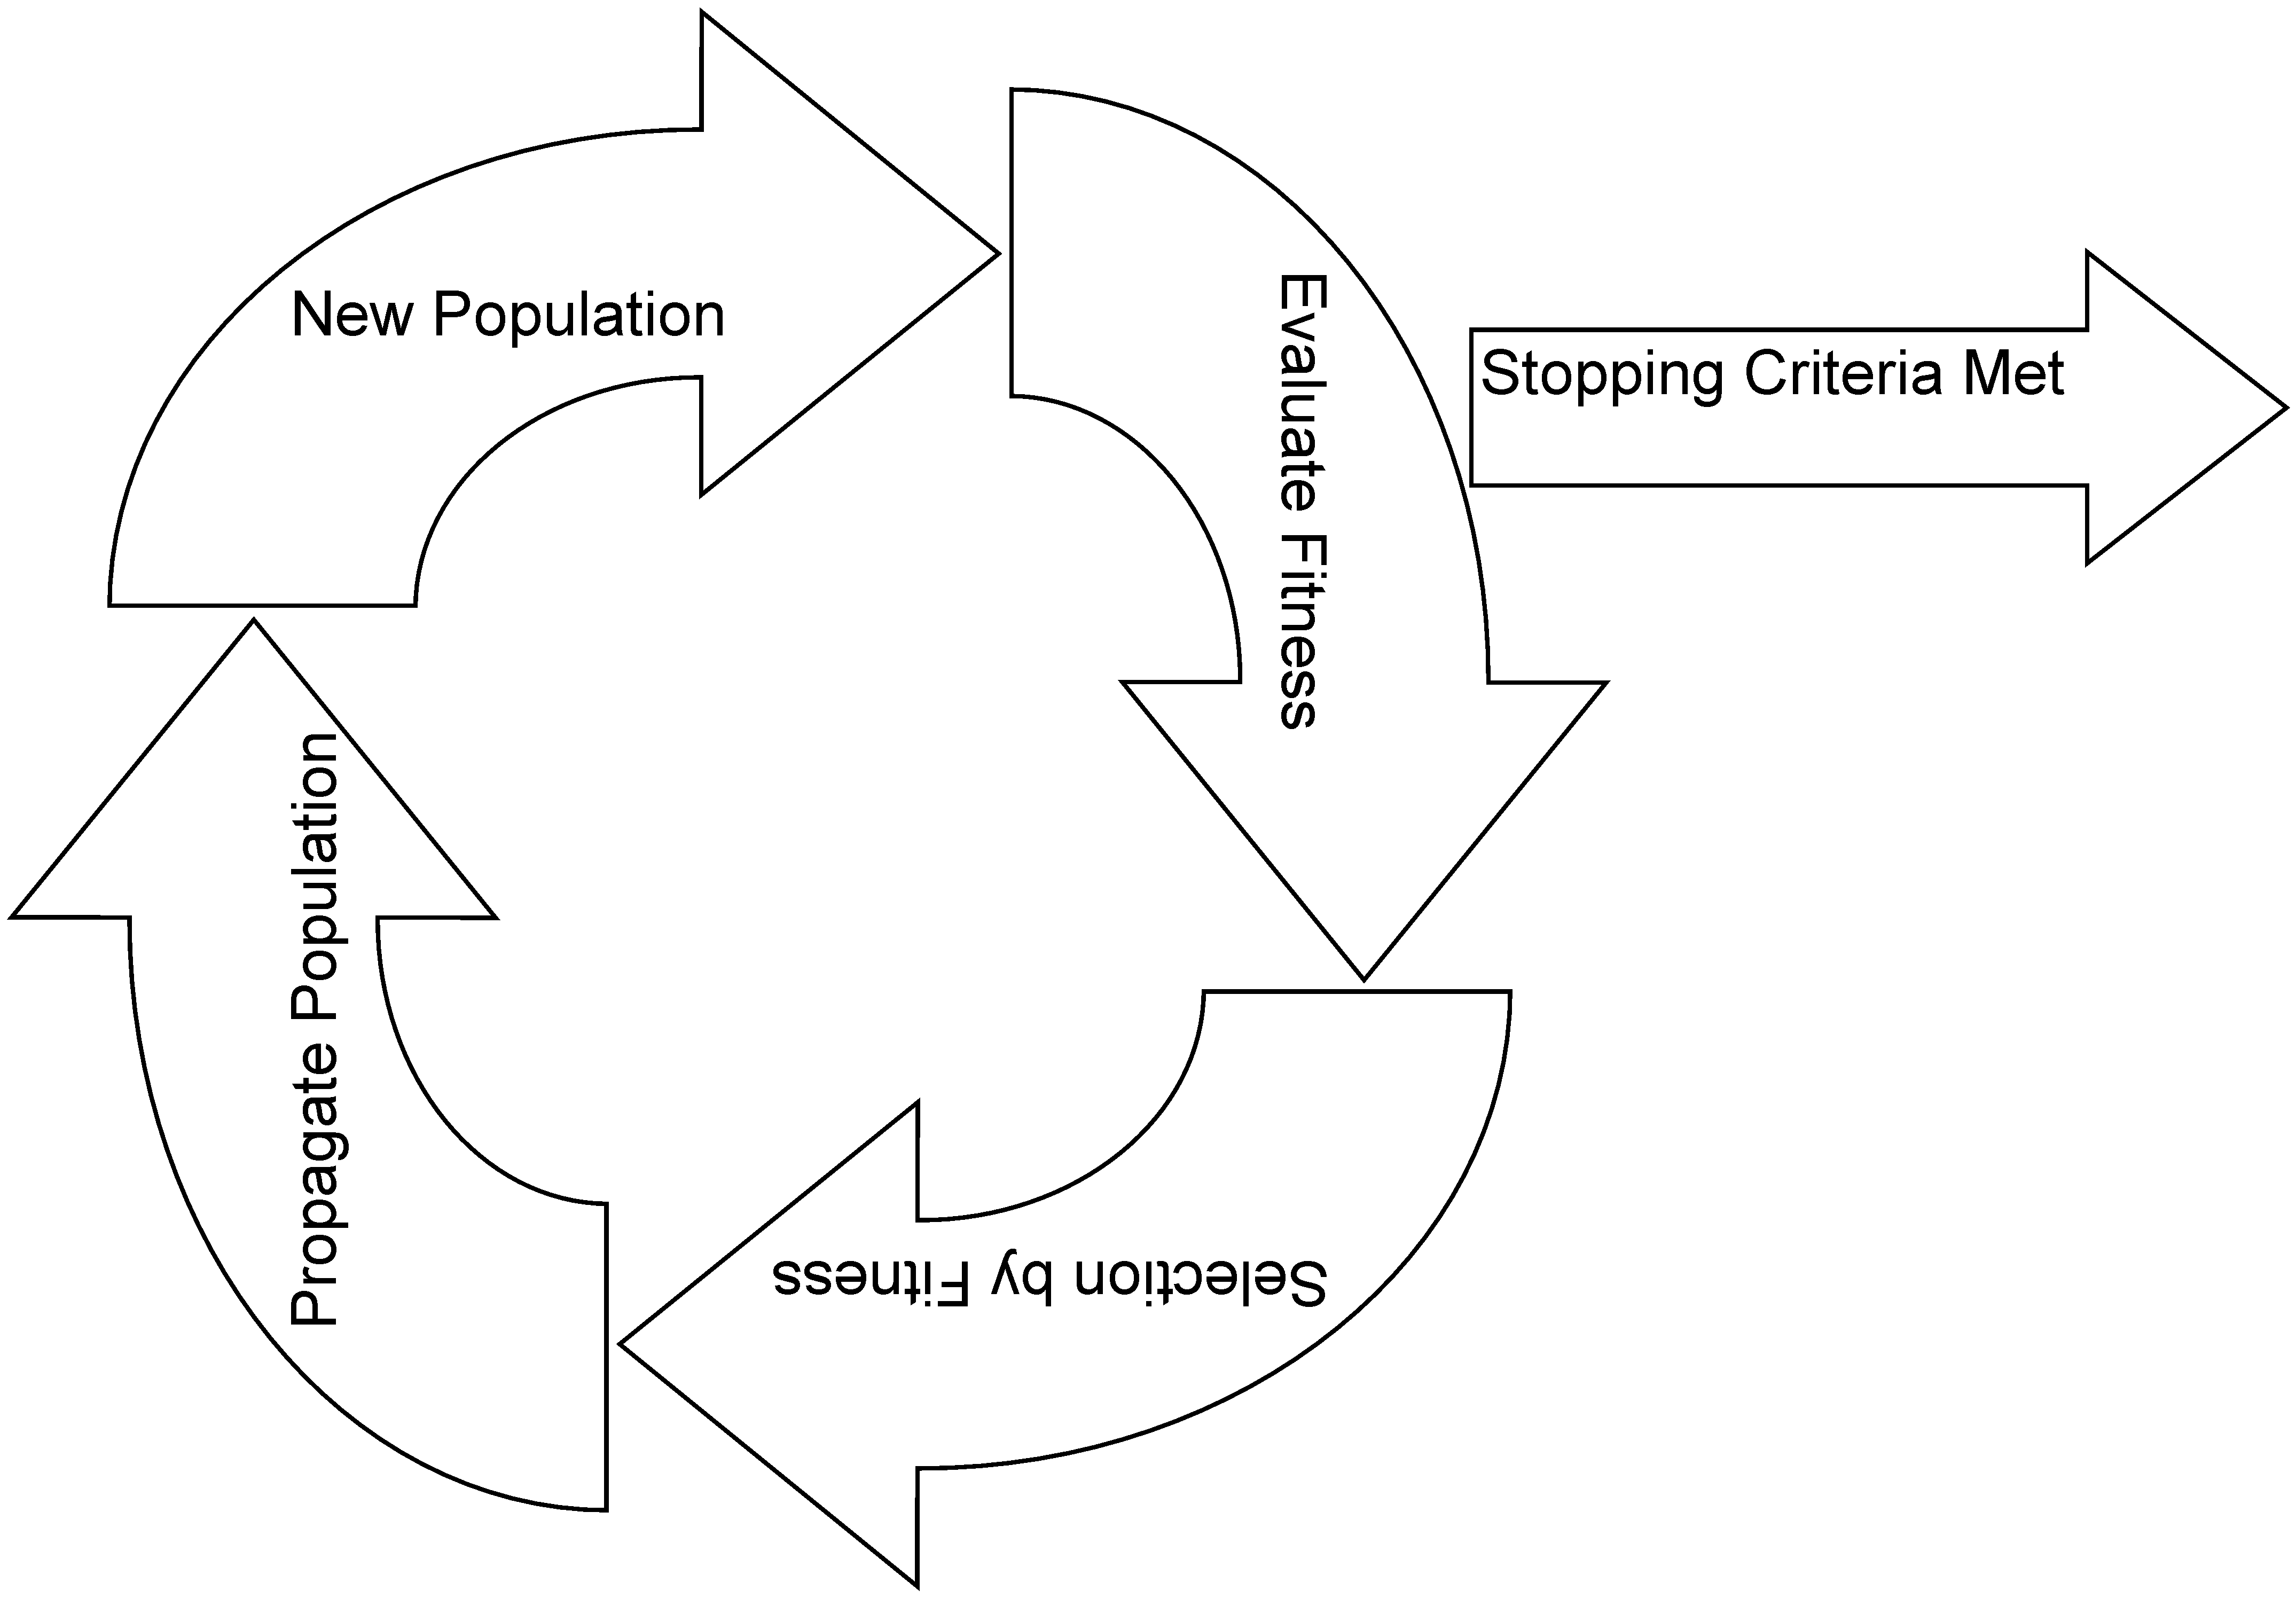
\includegraphics[width=1.0\columnwidth]{Figures/GAFlow.png}}
\caption[Genetic Algorithm Flow]{The general flow of a genetic algorithm. For a
computational genetic algorithm, the process is entered with New Population.
The fitness of the population is then evaluated. If the stopping criteria is
reached, the process is exited. Otherwise, individuals are selected for
propagation based on their fitness. A new population is propagated from
selected individuals using various techniques and a new population is created.}
\label{figure-gaflow}
\end{figure}

\subsection{New Population}

Applying a genetic algorithm to a problem requires that a solution to the
problem can be encoded into a data structure. A single data structure is
referred to as a chromosome. A given chromosome represents a single individual
in the population. In its simplest form a chromosome might consist of a binary
string, that is, a string of 1s and 0s~\cite{Holland1992,goldberg1989genetic}.
The interpretation of the chromosome is problem dependent. If the problem domain
is creating a melody, the 0s and 1s in the chromosome might encode specific
notes and other musical features; if the problem domain is the traveling
salesman problem, substrings in the chromosome might represent the cities that
are visited; if the problem domain is the set of moves in a game, substrings in
the chromosome might represent a particular game move.

The genetic algorithm for any problem begins by initializing the chromosomes
that represent solutions. This is usually done by randomly generating the data
in the chromosome. An individual chromosome is often referred to as an
individual and the complete set of chromosomes is referred to as the population.

The size of the population is an important decision in applying genetic
algorithms to a problem. A population that is too small may not find a solution,
or may take a long time to find a solution, which is a waste of computing
resources. A population that is too large may find a solution, but may use more
resources than is necessary.

\subsection{Fitness}

After a population of solutions is encoded, the next step is usually to measure
the fitness of the solution. Some kind of function is applied to each
chromosome, and the value of the function becomes the fitness of the 
chromosome~\cite{haupt2004practical}.

If the problem domain is creating a melody, the fitness function might be a
comparison of the melody encoded by the chromosome to the desired melody (which
is an objective fitness function) or it may be a human subjective judgement of
the melody; if the problem domain is the traveling salesman problem, the fitness
function would be the length of the tour encoded by the chromosome; if the
problem domain is the set of moves in a game, the fitness function could be the
payoff for making the move specified by the chromosome.

\subsection{Stopping Criteria}

After fitness is measured, the algorithm evaluates whether to stop or not. One
can stop after finding an exact solution, after solutions stop improving, or
after a set number of generations~\cite{dejong2006evolutionary}.

Obviously, if the algorithm has found an exact solution to a problem, there is
no point in proceeding further. This is often the case when optimizing a
mathematical function. If one knows ahead of time that the minimum or maximum of
a function is a particular value, and a genetic algorithm finds a solution that
produces that minimum or maximum, then if there is no reason to search for
additional solutions, the algorithm can terminate.

More often, though, the optimal fitness value is not known a priori. In this
case, one can measure the improvement in fitness between generations and stop
the algorithm when the solutions stop improving or when the improvement in
fitness between generations drops below some threshold.

A third criterion for stopping a genetic algorithm is when a preset number of
populations have evolved. Computer resources can be constrained, and although
an algorithm might find the optimal solution given enough CPU time, one can 
decide before starting the algorithm to terminate after \(n\) generations, and
take the best solution at that point.

\subsection{Selection}

After fitness is measured, the fitness is used to guide the selection of
individuals for propagation into the next
generation~\cite{haupt2004practical,dejong2006evolutionary}.

One method for performing this is to assign a weight to each individual
equal to the ratio of the individual's fitness to the total fitness of the
population. Then each individual is selected with probability equal to that
ratio. This is commonly referred to as roulette wheel selection. Another
technique is to randomly pick two individuals and compare their fitness; the
individual with the higher fitness is then selected. This is referred to as
tournament selection. 

Individuals that are selected can be moved directly into the next generation.
Alternately, they can be combined with other individuals to create new
individuals for the next generation. Either or both of those occur in the
propagation phase.

\subsection{Propagation}

Propagation of the current population usually occurs in conjunction with the
selection phase. The most common methods for creating a new population from the
current population are reproduction, recombination, and
mutation~\cite{goldberg1989genetic,haupt2004practical,DeJong:1989:UGA:93126.93172}.

In reproduction, individuals are copied from the current population directly
into the new population. This might consist of choosing the highest quality
solutions and copying them (elitism) or individuals might be chosen in the
selection phase for copying.

In recombination, two individuals are chosen in the selection process, and then
these two individuals are recombined in some way to create new child
individuals. The most common method of recombination is known as crossover. For
crossover, two individuals are selected and then a position in the chromosome is
randomly chosen, the chromosome is split at that point, and then one of the
sections created is exchanged with the same section in the other chromosome.
This creates two new individuals in the new population. There are other
techniques for recombination; those will be discussed in
Section~\ref{2-recombination}.

In mutation, an individual is selected and the chromosome of the individual is
randomly changed. This can be an individual in the current population; the
mutated individual is then placed in the new generation. Alternately it can be
one of the child individuals created through recombination that is mutated.

After the new population is created, the process repeats.

\section{Genetic Algorithm Extensions}

A large amount of research has been conducted into extending various features of
the basic algorithm to cover a larger number of problems. We briefly look at
some of those extensions here, with additional coverage of specific fitness
measurement extensions in Chapter~\ref{chap:background}.

\subsection{Chromosomes}

The chromosomes in genetic algorithms were introduced above as a binary string.
However, the chromosome is, more generally, some data structure that represents
the solution to some problem. So one can have chromosomes that are strings or
arrays of integers, arrays of real numbers, or strings or arrays of some other
encoding~\cite{haupt2004practical}. Chromosomes can be structured as trees,
where nodes and leaves represent some part of the solution. These are usually
used in genetic programming where the tree is the parse tree of some computer
program and the objective is to evolve a program~\cite{koza1992genetic}.
Chromosomes can be used to represent graph-like structures such as finite state
machines~\cite{fogel1999intelligence,fogel2000evolutionary}. Linear chromosomes
that are translated into gene expression trees are used in gene expression
programming~\cite{ferreira2012gene}.

\subsection{Fitness evaluation}

The fitness function is used to evaluate the quality of the solution. Thus, it
is better to have some objective function or measurement that can be applied to
the chromosome. When attempting to optimize some mathematical function, that is
easy to do. The chromosome becomes an input to the function, and the objective
measure is simply the function output. For other problems, though, there may not
be an objective function. For example, when applying a genetic algorithm to art
or music, a subjective fitness function is used~\cite{eiben2003introduction}.
For these applications a human is usually used to provide an assessment of the
quality of the solution.

And then there are times when there is neither an objective nor a subjective
fitness function. When applying genetic algorithms to games, especially games
that have a stochastic component, there is no good objective fitness function.
If a chromosome is designed to output moves for a game, how does one know
whether the strategy encoded by the chromosome is a good? Just because an
individual wins a game does not make the individual high quality: it could be a
poor quality individual but played against a worse player. Similarly, just
because an individual loses a game does not make the individual poor quality: it
could have lost just because of chance. In this case, one uses a competitive
fitness function~\cite{fogel1999intelligence}. We discuss competitive fitness 
functions in more detail in Chapter~\ref{chap:background}.

\section{Recombination and mutation} \label{2-recombination}

There are many different ways to perform recombination in a genetic algorithm.
The basic crossover operation was briefly discussed earlier. When recombining
strings or arrays, one can also use multi-point crossover where multiple
crossover points are used. In uniform crossover each gene in the child is
randomly selected from the parents. With real-valued or continuous chromosomes,
there is arithmetic (also known as blended) crossover that linearly combines
both parent chromosomes to create two child
chromosomes~\cite{haupt2004practical}. With a problem like the traveling
salesman problem, the standard crossover operations are not appropriate since
they can duplicate cities in the chromosome. For permutation type problems like
the traveling salesman problem, other crossover operations have been
developed~\cite{goldberg1989genetic} which avoid duplications in the child
chromosomes.
